%%%%%%%%%%%%%%%%%%%%% chapter.tex %%%%%%%%%%%%%%%%%%%%%%%%%%%%%%%%%
%
% sample chapter
%
% Use this file as a template for your own input.
%
%%%%%%%%%%%%%%%%%%%%%%%% Springer-Verlag %%%%%%%%%%%%%%%%%%%%%%%%%%
%\motto{Use the template \emph{chapter.tex} to style the various elements of your chapter content.}
\chapter{Requirements and Regulations in the $5$ GHz Unlicensed Spectrum}
\label{sec:LBT-overview} 

\abstract*{Licenses and fees are not required for operators to use the $5$ GHz unlicensed spectrum. However, in order to avoid interference and to ensure a fair use of this resource, numerous requirements and regulations are imposed by national and international organizations. When operating in this band, the emerging \mbox{U-LTE} technology, needs to adhere to these regulations, as any other existing technologies, esp., IEEE 802.11/\mbox{Wi-Fi}, would. This chapter provides an overview on the radio spectrum resources in these bands and the related management and allocation concerns. It then summarizes a number of the key requirements and regulations specified by the European Telecommunications Standards Institute (ETSI) and the Federal Communications Commission (FCC) on radio channels, operating channel selection, transmission power, and channel access rules. These technical details are the baselines to be followed when designing medium access control protocols for \mbox{U-LTE} and any other technologies operating in the $5$ GHz unlicensed radio band.}

Licenses and fees are not required for operators to use the $5$ GHz unlicensed spectrum. However, in order to avoid interference and to ensure a fair use of this resource, numerous requirements and regulations are imposed by national and international organizations. When operating in this band, the emerging \mbox{U-LTE} technology, needs to adhere to these regulations, as any other existing technologies, esp., IEEE 802.11/\mbox{Wi-Fi}, would. This chapter provides an overview on the radio spectrum resources in these bands and the related management and allocation concerns. It then summarizes a number of the key requirements and regulations specified by the European Telecommunications Standards Institute (ETSI) and the Federal Communications Commission (FCC) on radio channels, operating channel selection, transmission power, and channel access rules. These technical details are the baselines to be followed when designing medium access control protocols for \mbox{U-LTE} and any other technologies operating in the $5$ GHz unlicensed radio band.

\section{Radio Spectrum Management: An Overview}

The Radio Frequency (RF) spectrum is the part of the electromagnetic spectrum from $3$ Hz to $3000$ GHz ($3$ THz). Radio waves in this frequency range are widely used in modern technologies, especially in telecommunications. The radio spectrum is divided into different chunks or bands, each of which can be used by one or multiple technologies. Radio Frequency Interference (RFI) can disrupt and disturb the normal functioning of devices, and thus it is always important to avoid or keep the RFI within acceptable levels. For this, the generation and transmission of radio waves is strictly regulated by national laws, coordinated by international organizations, e.g., Federal Communications Commission (FCC), Inter-American Telecommunication Commission (CITEL), International Telecommunication Union (ITU), European Telecommunications Standards Institute (ETSI), etc. 

Most countries consider RF spectrum as a national resource. The process of regulating the use of this resource is spectrum management or allocation. Spectrum allocation varies by country and/or regulatory domain. In United States, for example, the FCC regulates inter-state communications by radio, television, wire, satellite, and cable in all states and territories. From a management perspective, radio bands are categorized into \textit{licensed} and \textit{unlicensed}. Licensing is a way of ensuring that wireless operators do not interfere with each others by giving each of them the exclusive use of one or more bands in given geographical areas, over a set period of time. Licensed bands are mainly sold or assigned to operators through  a spectrum auction process. These licensed spectrum allocations are primarily used by the television broadcasting, commercial radio, and cellular voice and data industries. Operating in their own licensed bands, operators can avoid RFI from other users and thus guarantee the quality of services they deliver to their subscribers. However, licensing would be very impractical for certain use cases, like communications between cordless handsets and base units. Instead, such wireless technologies transmits its radio signals in unlicensed frequency bands - usually the Industrial, Scientific and Medical (ISM) band defined by the ITU radio regulations and allocated in most countries for free use by anyone without any licenses and fees. Unlicensed bands enable numerous technologies and products, e.g., \mbox{Wi-Fi}, Bluetooth, and many other low-power short-range communications technologies. These bands are open sandboxes where users can operate without the high barriers to entry, such as costs, that are seen in the licensed spectrum bands. The availability of unlicensed bands provides a platform for innovation, a greenfield space for technology start-ups and entrepreneurs, as well as established companies. Internet of Things (IoT)---the development and deployment of networking technologies that provide connectivity to everyday objects for many innovative applications--is fundamentally enabled by unlicensed spectrum.

Today, most people are within a few meters of consumer products (e.g, microwave ovens, \mbox{Wi-Fi}, Bluetooth, etc.) that use the unlicensed bands. In other words, there is a great chance for RFI in these bands. As a result, even though no permission is required for the use of unlicensed bands, manufacturers and users must comply with numerous rules and regulations (related to transmission power, transmission time, etc.) in order to minimize the RFI to others as well as to ensure a fair sharing of the radio resource in these bands. IEEE 802.11/\mbox{Wi-Fi} is the most successful and popular technology operating in unlicensed spectrum. \mbox{Wi-Fi} manufacturers need to obtain compliance certifications from \mbox{Wi-Fi} Alliance whose certification program is designed following rules imposed by radio spectrum management organizations/authorities such as ETSI and FCC. 

The two most widely-used unlicensed bands are $2.4$ GHz and $5$ GHz. These two bands have their own advantages and disadvantages in various perspectives. $5$ GHz provides faster data rates at a shorter distance, whereas $2.4$ GHz offers coverage for greater distances but supports lower rates. New technologies, particularly unlicensed LTE variants including \mbox{LTE-U}, \mbox{LAA-LTE}, and MulteFire, as mentioned in Chapter \ref{intro}, have been targeted to operate in the $5$ GHz band alongside \mbox{Wi-Fi}. The selection of the $5$ GHz band for \mbox{U-LTE} technologies (rather than the $2.4$ GHz band) is mainly due to the following reasons:
\begin{itemize}
\item
\textit{More available channels:} In the $2.4$ GHz band, only $14$ channels, each of with provides $20$ MHz of bandwidth, are defined. In U.S. (or Europe), only $11$ (or $13$) of those channels are legally available. However, those channels overlap excessively with one another. Due to this overlapping, the maximum possible number of parallel independent connections is limited to $3$ channels (channels $1$, $6$, and $11$). In the $5$ GHz band, there are $21$ non-overlapping $20$ MHz channels (or $9$ non-overlapping $40$ MHz channels). Fig. \ref{figs:2-5GHz-spectrum} depicts spectrum analyzer views of radio channels defined in $2.4$ and $5$ GHz bands, respectively.
\item
\textit{Lower level of interference:} Since the $2.4$ ISM band was released for \mbox{Wi-Fi} technology use more than fifteen years ago, this band is over-crowded with billions of existing \mbox{Wi-Fi} devices. There are also many consumer products which use this band, including microwave ovens, cordless phones, baby monitors, garage door openers, etc. In contrast, the relatively recent release of the $5$ GHz band for private use makes this band much less crowded and thus having a much lower level of RFI. 
\item
\textit{Higher performance:} The $5$ GHz band operates on a larger spectrum and does not suffer the over-crowding. Therefore, compared to the $2.4$ GHz band, each channel in the $2.4$ GHz band allows for much better spectrum efficiency and higher data rates.
\end{itemize}
\begin{figure}[!ht] 	
	\subfloat[2.4 GHz band]{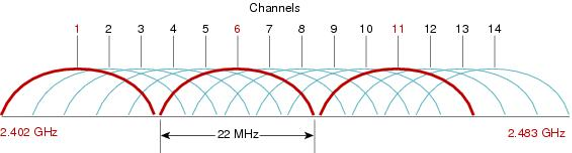
\includegraphics[width=\textwidth]{figs/2-4GHz}%
		\label{figs:2GHz-spectrum}}
	\\
	\subfloat[5GHz band]{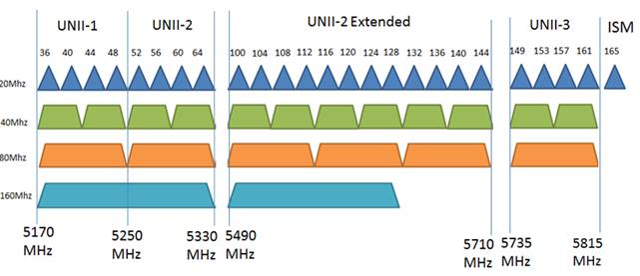
\includegraphics[width=\textwidth]{figs/5GHz}%
		\label{5GHz-spectrum}}
	\caption{$2.4$ GHz and $5$ GHz Unlicensed Spectrums.}
	\label{figs:2-5GHz-spectrum}
\end{figure}

As mentioned, any technology operating in unlicensed bands needs to comply with existing rules and regulations in order to limit RFI and to ensure that it does not unfairly grab a larger portion of the shared spectrum.  Coexistence is one of the most notable concerns when \mbox{U-LTE} technology is introduced into the $5$ GHz unlicensed band considering the sheer number of \mbox{Wi-Fi} devices and networks that have been deployed in the same band for everyday applications in homes, offices, and campuses. Since the number of wireless devices using the $5$ GHz band has grown rapidly over the last few years, ETSI has updated its related regulations. For background knowledge necessary for developments of radio channel access protocols for \mbox{U-LTE} and \mbox{Wi-Fi} technologies in this band, the following sections summarize a number of key requirements and mechanisms presented in ETSI EN 301 893. Specifically, the available frequency channels, transmission power, and channel access mechanisms are explained in detail.

\section{Frequency Channels}

The ETSI EN 301 893 V1.7.2 regulations \cite{LBT-ETSI-2014} released in July 2014 define three unlicensed frequency bands:
\begin{itemize}
\item
	RLAN band 1: $5150$ to $5350$ MHz, divided into 2 sub-bands
	\begin{itemize}
	\item
		Sub-band I: $5150$ MHz - $5250$ MHz. This sub-band is comparable to FCC U-NII-1. 
	\item
		Sub-band II: $5250$ MHz - $5350$ MHz. This sub-band is comparable to FCC U-NII-2.
	\item
		RLAN band 2: $5470$ MHz - $5725$ MHz. This band comparable to FCC U-NII-2 extended (U-NII-2e).
	\item
		RLAN band 3, also known as Broadband Radio Access Networks (BRAN): $5725$ – $5875$ MHz. This sub-band is comparable to FCC U-NII-3 ($5725$ – $5825$ MHz) band with a higher upper frequency range.
	\end{itemize}
\end{itemize}

The radio channels defined in the $5$ GHz band by ETSI 301 893 standard (with a reference to FCC regulations) are summarized in Fig. \ref{5GHz-spectrum}.  Technical details and the availability of each channel in four main regions (U.S., Europe, Japan, and China) are presented in Fig. \ref{figs:5GHz-spectrum-table}.
\begin{figure}[!ht]
	\centering
	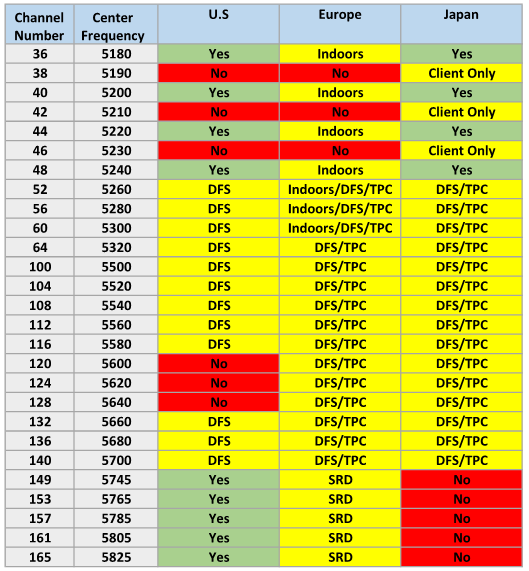
\includegraphics[width=0.9\columnwidth]{figs/5GHz-spectrum-table}
	\caption{Details of $5$ GHz Unlicensed Channels in Different Regions.}
	\label{figs:5GHz-spectrum-table}
\end{figure}


\section{Transmission Power}

Each of the bands defined by ETSI EN 301 893 V1.7.2 regulations \cite{LBT-ETSI-2014} have different maximum allowable transmission power levels. Note that the RF output power is defined as the mean Equivalent Isotropic Radiated Power (EIRP) of the equipment during a transmission burst. In general, the limits are valid for the device with antenna gain and cable loss and not only the output power of WLAN module.

\subsection{RLAN band 1 ($5150$ to $5350$ MHz)} 

\subsubsection{Indoor only Sub-band I ($5150$ - $5250$ MHz)}
The first RLAN sub-band includes the channels $36$ to $48$ and has an EIRP power limit to $23$ dBm ($200$ mW). These channels are considered for indoor only usage and do not require any Dynamic Frequency Selection (DFS) or Transmit Power Control (TPC) features. 

\subsubsection{Indoor only Sub-band II ($5250$ - $5350$ MHz)}
In the second sub-band of the RLAN band 1 with channels $52$ to $64$, ETSI has set the EIRP power limit to $23$ dBm ($200$ mW) for devices with TPC and $20$ dBm ($100$ mW) for devices without TPC. For a device with TPC, the mean EIRP at the lowest power level of the TPC range must not exceed $17$ dBm ($50$ mW). This band requires DFS support (and requires TPC support in Europe and Japan).

\subsection{RLAN band 2 ($5470$ to $5725$ MHz)}

Channels from $100$ to $140$ are part of the second RLAN band and have an EIRP power limit of $30$ dBm ($1000$ mW) for devices with DFS and TPC support, $27$ dBm ($500$ mW) for non-TPC devices, and $20$ dBm ($100$ mW) for devices with neither TPC or DFS support. The mean EIRP power level for a slave device with TPC must not exceed $24$ dBm at the lowest TPC power level if the device is also capable of radar detection or $17$ dBm otherwise. 

\subsection{BRAN ($5725$ to $5875$ MHz)} 

ETSI has restricted the channels $155$ to $171$ for Broadband Wireless Access (BWA) use only. The idea is to provide internet access to locations without any wired access network available. The maximum EIRP output power has been set to $36$ dBm ($4000$ mW) with the limitation of RF power into antenna of $30$ dBm ($1000$ mW).


\section{Transmission Power Control (TPC)}

Dynamic adjustment of the transmission power is intended to reduce RFI. Dynamically adjusting the transmission power facilitates the shared use of the $5250$-$5350$ MHz and $5470$-$5725$ MHz frequency bands with satellite services. TPC determines the minimum transmission power necessary to maintain the connection with the partner (such as an access point).

If TPC is not used within these frequency bands, then the highest permissible average EIRP and the corresponding maximum EIRP density are reduced by $3$ dB. This restriction does not apply to the frequency range of $5150$-$5350$ MHz. Without DFS and TPC, a maximum of only $30$ mW EIRP is permitted. When DFS and TPC are used, a maximum $1000$ mW EIRP is permitted as the transmission power (compared with $100$ mW with 802.11 b/g, $2.4$ GHz, DFS and TPC are not possible here). The higher maximum transmission power not only compensates for the higher attenuation of $5$ GHz radio waves in air, it also makes noticeably longer ranges possible than in the $2.4$ GHz range. 


\section{Dynamic Frequency Selection (DFS)}

DFS was stipulated to (i) detect interference from radar systems (radar detection) and to avoid co-channel operation with these systems; and (ii) to provide, on aggregate, a near-uniform loading of the spectrum (Uniform Spreading). DFS is stipulated for the frequency ranges of $5250$-$5350$ MHz and $5470$-$5725$ MHz. It is optional for the frequency range of $5150$-$5250$ MHz.

DFS initially assumes that no channel is available in the corresponding frequency band. The WLAN device selects an arbitrary channel at the start and performs what is known as a Channel Availability Check (CAC). Before transmitting on a channel, a Channel Observation Time (COT) of $60$ seconds is observed to allow a check to see if a different device is already working on this channel and the channel is therefore occupied. If th channel is occupied, then a different channel is checked by the CAC. If not, then the WLAN device can perform its transmission operation. Even during operation, a check is run to see if a primary application such as a radar device is using this channel. This exploits the fact that radars frequently work according to the rotation method, whereby a tightly bundled directional transmission signal is transmitted by a rotating antenna. A remote receiver perceives the radar signal as a short pulse (radar peak). If a device receives such a radar peak, it pauses the transmission operation and monitors the channel for further pulses. If additional radar peaks occur during the COT, then a new channel is selected automatically. A check of this type is required to be carried out every $24$ hours. This is why interrupting the data transmission for $60$ seconds is unavoidable. 


\section{Channel Access Mechanisms}
\label{subsec:ETSI-overview}

In order to avoid channel collisions when two or more than two devices transmit the signal in the same channel at the same time, Listen Before Talk (BLT) strategy is employed. ETSI EN 301 893 V1.7.2 \cite{LBT-ETSI-2014} describes two mechanisms that require an equipment or a device to apply CCA before using the channel. The first mechanism is Frame Based Equipment (FBE) which defines a fixed (not directly demand-driven) timing frame for channel access. The second mechanism is Load Based Equipment (LBE) which defines demand-driven timing frame.

\subsection{FBE-based Mechanism}
\label{etsi-lbt:fbe}

A simplified flowchart and an illustrative example of the channel access procedure used for FBE are given in Figs. \ref{figs:FBE-flowchart} and \ref{figs:FBE-example}, respectively.
\begin{figure}[!ht]
	\centering
	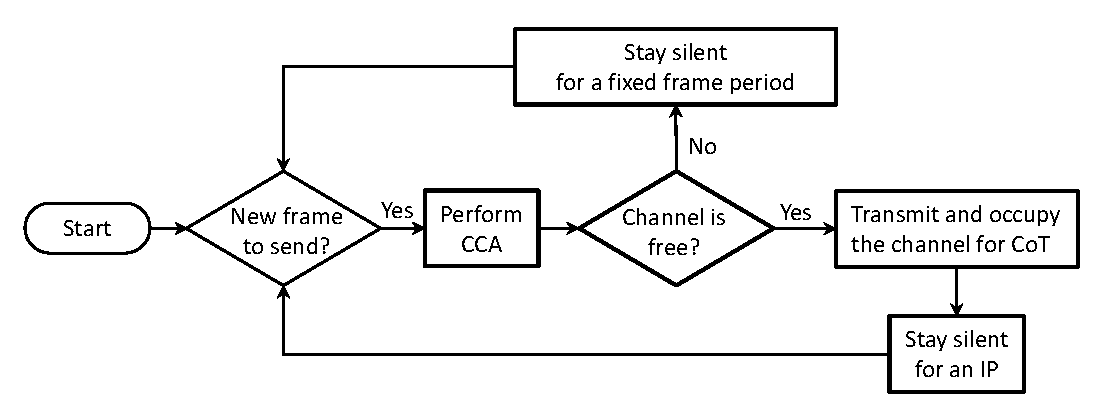
\includegraphics[width=0.9\columnwidth]{figs/FBE-flowchart}
	\caption{Simplified flowchart of FBE.}
	\label{figs:FBE-flowchart}
\end{figure}
\begin{figure}[!ht]
	\centering
	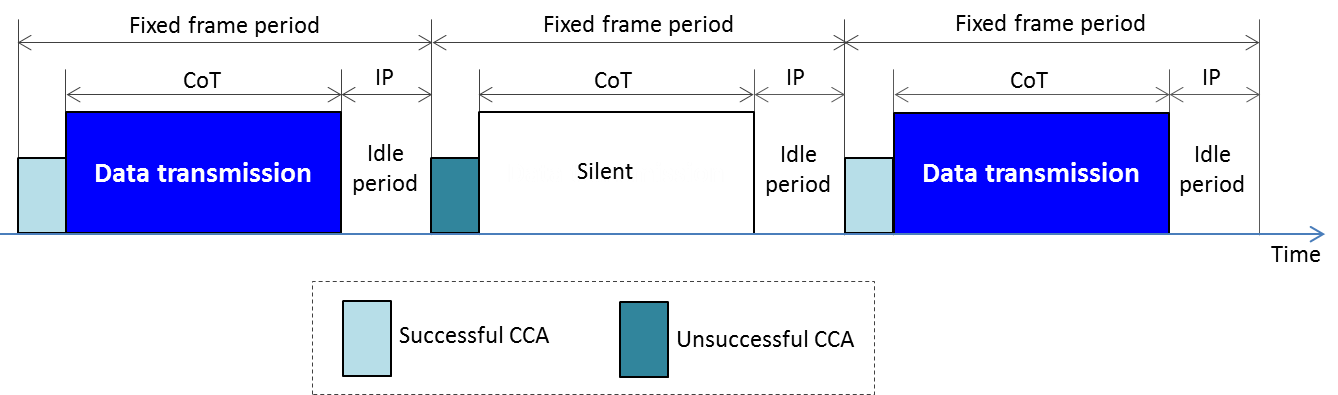
\includegraphics[width=0.9\columnwidth]{figs/FBE-example}
	\caption{An illustrative example of FBE.}
	\label{figs:FBE-example}
\end{figure}


\noindent FBE shall comply with the following requirements:

\begin{itemize}
	
	\item
	\textit{R1:} Before starting transmissions on an operating channel, the equipment shall perform a CCA check using Energy Detect (ED). The equipment shall observe the channel for the duration of the CCA observation time. The operating channel shall be considered occupied if the energy level in the channel exceeds the threshold corresponding to the power level.
	
	\item
	\textit{R2:}
	If the CCA procedure finds that the channel is clear, the equipment may transmit immediately and occupy the channel for a fixed time period.
	
	\item
	\textit{R3:} If the CCA procedure finds that the channel is occupied, the equipment shall not transmit on that channel during the next fixed frame period.
	
	\item
	\textit{R4:} The total time during which an equipment has transmissions on a given channel without re-evaluating the availability of that channel is defined as the \textit{Channel Occupancy Time} (CoT).
	
	\item
	\textit{R5:} After occupying the channel for CoT, the equipment keeps silent and waits for a short time, namely \textit{Idle Period} (IP).
	
	\item
	\textit{R6:} Towards the end of the idle period, the equipment shall perform a new CCA procedure as described in R1 above.
	
	\item
	\textit{R7:} The equipment, upon correct reception of a packet which was intended for this equipment, can skip CCA and immediately proceed with the transmission of management and control frames, e.g., acknowledgement (ACK) and block ACK frames.
	
	\item
	\textit{R8:}
	A consecutive sequence of such transmissions by the equipment, without it performing a new CCA, shall not exceed the maximum CoT.
	
	\item
	\textit{R9:}
	CCA observation time shall be not less than $20$ $\mu$s.
	
	\item
	\textit{R10:} CoT shall be in the range from $1$ ms to $10$ ms.
	
	\item
	\textit{R11:}
	The minimum IP shall be at least $5$\% of CoT used by the equipment for the current fixed frame period.
	
\end{itemize}


\subsection{LBE-based Mechanism}
\label{etsi-lbt:lbe}

A simplified flowchart and an illustrative example of the channel access procedure used for LBE are given in Figs. \ref{figs:LBE-flowchart} and \ref{figs:LBE-example}, respectively.
\begin{figure}[!ht]
	\centering
	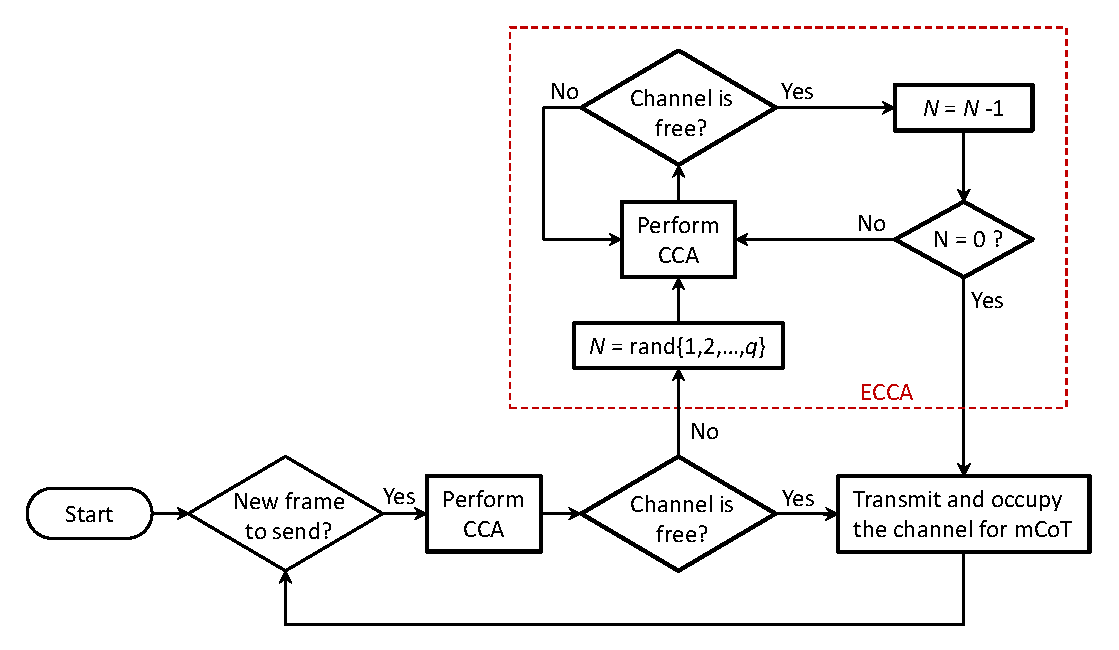
\includegraphics[width=0.9\columnwidth]{figs/LBE-flowchart}
	\caption{Simplified flowchart of LBE.}
	\label{figs:LBE-flowchart}
\end{figure}
\begin{figure}[!ht]
	\centering
	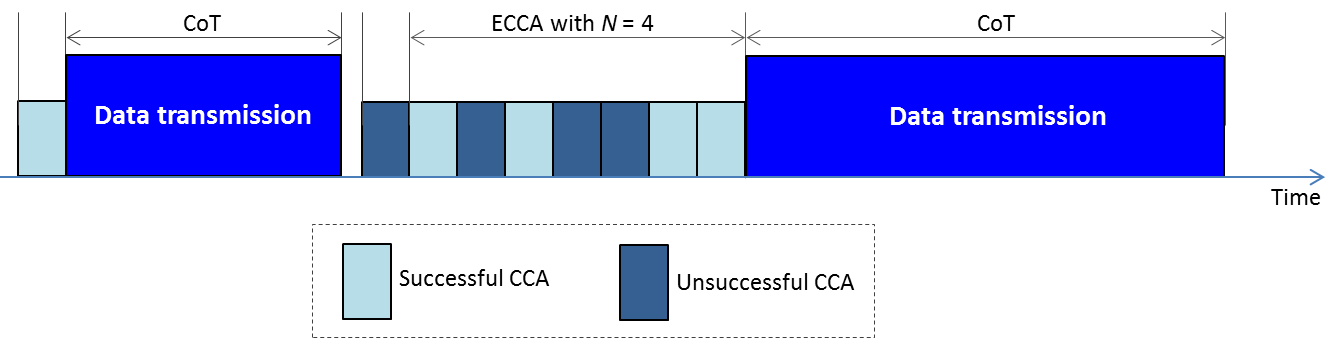
\includegraphics[width=0.9\columnwidth]{figs/LBE-example}
	\caption{An illustrative example of LBE.}
	\label{figs:LBE-example}
\end{figure}


\noindent LBE shall comply with the following requirements:

\begin{itemize}
	
	\item
	\textit{R1:} Before starting transmissions on an operating channel, the equipment shall perform a CCA check using ED. The equipment shall observe the channel for the duration of the CCA observation time. The operating channel shall be considered occupied if the energy level in the channel exceeds the threshold corresponding to the power level.
	
	\item
	\textit{R2:}
	If the CCA procedure finds the that channel is clear, the equipment may transmit immediately on that channel.
	
	\item
	\textit{R3:}
	If the CCA procedure finds that the channel is occupied, it shall not transmit in that channel. The equipment shall perform an Extended CCA (ECCA) procedure in which the channel is observed for a random duration.
	
	\item
	\textit{R4:}
	If the ECCA procedure has determined the channel to be clear, the equipment may initiate transmissions on this channel.
	
	\item
	\textit{R5:}
	The total time that an equipment makes use of the channel (without performing CCA) is the maximum Channel Occupancy Time (mCoT), after which the device shall perform a new CCA procedure as described in R1 above.
	
	\item
	\textit{R6:}
	The equipment, upon correct reception of a packet which was intended for this equipment, can skip CCA and immediately proceed with the transmission of management and control frames, e.g., ACK and block ACK frames.
	
	\item
	\textit{R7:}
	A consecutive sequence of transmissions by the equipment, without it performing a new CCA, shall not exceed mCoT.
	
	\item
	\textit{R8:}
	CCA observation time shall be not less than $20$ $\mu$s.
	
	\item
	\textit{R9:}
	The random duration in an ECCA procedure is $N \times$ (CCA observation time), where $N$ is randomly selected in the range $\{1,2,...,q\}$, $q \in \{4,5,...,32\}$ (declared by the manufacturer).
	
	\item
	\textit{R10:}
	mCoT should be less than $(13/32)\times q$ ms (mCoT is in the range from $1.625$ to $13$ ms).
	
\end{itemize}

%%%%%%%%%%%%%%%%%%%%%%%% referenc.tex %%%%%%%%%%%%%%%%%%%%%%%%%%%%%%
% sample references
% %
% Use this file as a template for your own input.
%
%%%%%%%%%%%%%%%%%%%%%%%% Springer-Verlag %%%%%%%%%%%%%%%%%%%%%%%%%%

\begin{thebibliography}{99.}%
\bibitem{LBT-ETSI-2014}
\emph{ETSI EN 301 893 V1.7.2 (2014-07): Broadband Radio Access Networks (BRAN); 5 GHz high performance RLAN; Harmonized EN covering the essential requirements of article 3.2 of the R\&TTE Directive}, European Telecommunications Standards Institute Std., 2014.
\end{thebibliography}
